\documentclass{article}%
\usepackage[T1]{fontenc}%
\usepackage[utf8]{inputenc}%
\usepackage{lmodern}%
\usepackage{textcomp}%
\usepackage{lastpage}%
\usepackage[head=40pt,margin=0.5in,bottom=0.6in]{geometry}%
\usepackage{graphicx}%
%
\title{\textbf{Hospitales se quedan sin camas ni enfermeras}}%
\author{Olgalinda Pimentel R.}%
\date{28/09/2018}%
%
\begin{document}%
\normalsize%
\maketitle%
\textbf{URL: }%
http://www.el{-}nacional.com/noticias/sociedad/hospitales{-}quedan{-}sin{-}camas{-}enfermeras\_253524\newline%
%
\textbf{Periodico: }%
EN, %
ID: %
253524, %
Seccion: %
Sociedad\newline%
%
\textbf{Palabras Claves: }%
Salud, Crisis humanitaria, Sociedad\newline%
%
\textbf{Derecho: }%
2.1%
, Otros Derechos: %
NO\_TIENE%
, Sub Derechos: %
2.1.1%
\newline%
%
\textbf{EP: }%
NO\newline%
\newline%
%
\textbf{\textit{Un estudio realizado por el gremio de salud en 32 centros asistenciales, correspondiente al mes de septiembre, revela que la mayoría no presta regularmente servicios de laboratorio ni rayos X. Han cerrado 13 áreas de pediatría y 11 unidades de cuidados intensivos de adultos ~}}%
\newline%
\newline%
%
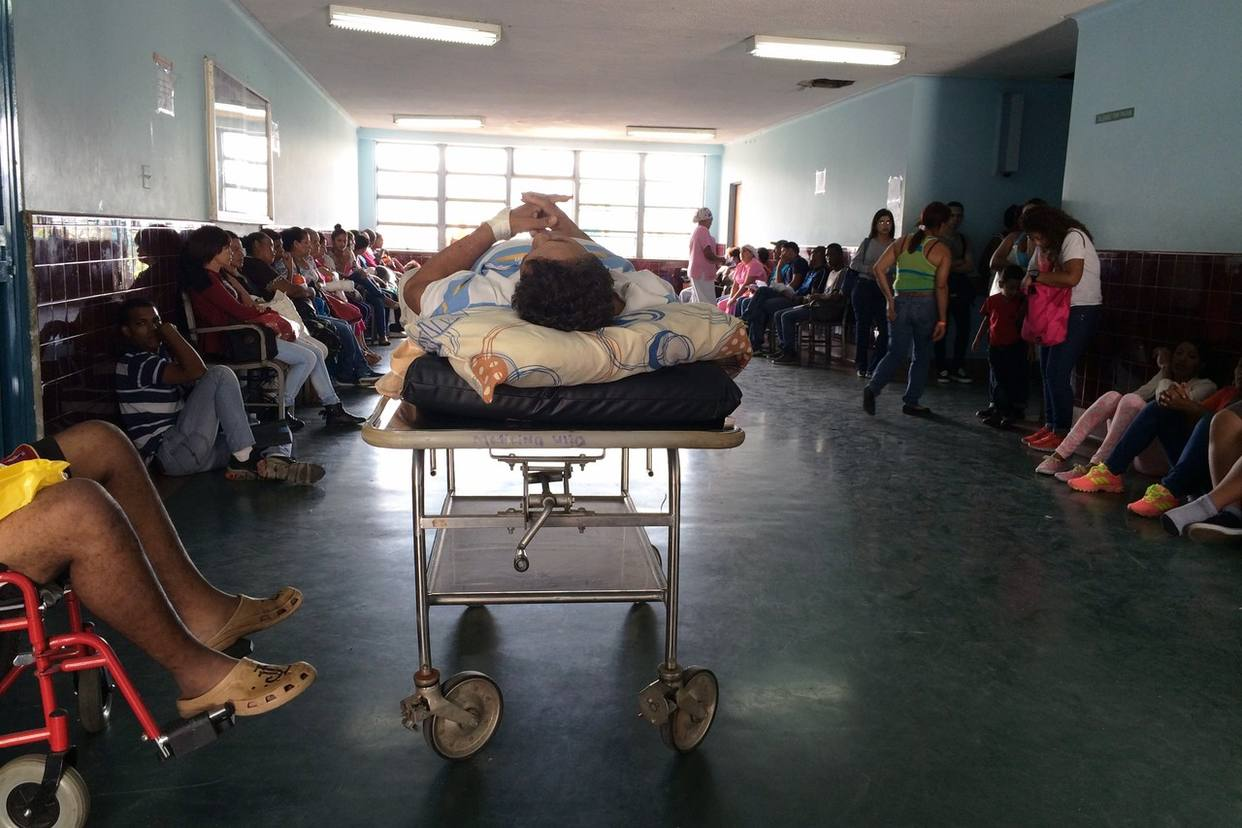
\includegraphics[width=300px]{118.jpg}%
\newline%
%
Las opciones de atención médica pública en Venezuela son cada vez más escasas. En 32 centros asistenciales del país, la mayoría tipo IV, es decir, de referencia, están operativas solo 6.330 camas de las 10.648 programadas, lo que significa que los hospitales tienen reducida en 40.55\% la capacidad de hospitalización.%
\newline%
%
Este es uno de los resultados preliminares de la Encuesta Nacional del sistema y la organización asistencial, realizada por el gremio entre los profesionales de la salud para evidenciar la magnitud de la crisis en el sector. En el estudio, en el cual participaron tres investigadores y una decena de colaboradores, se tomó una muestra inicial de 83 hospitales de los 23 estados y el Distrito Capital, y se procesó la respuesta obtenida en 38\% de los centros, 10 de ellos ubicados en Caracas. Del total consultado, 56,3\% es tipo IV, 78,1\% adscrito al Ministerio de Salud, y 15,6\% pertenece al IVSS.%
\newline%
%
De acuerdo con las respuestas, la mayoría no cuenta con analgésicos ni antibióticos, y tampoco con insumos médicos; las áreas de emergencia, quirófano y maternidad funcionan de modo intermitente, al igual que los servicios de laboratorio, rayos X y ecografía. En la investigación resalta que cerraron 13 áreas de pediatría y 11 unidades de cuidados intensivos de adultos.%
\newline%
%
La escasez de personal de salud ha ocasionado la clausura de servicios, señala el trabajo. De 12.113 enfermeras con las que contaba el sistema, renunciaron 6.030 y 5.106 se fueron del país.%
\newline%
%
Otro resultado indica que 56,3\% de los consultados afirmó que los hospitales presentan desmejoras de remuneración, y en las condiciones de trabajo hay jornadas extremas; así también se cita la falta de transporte y de dinero en efectivo.%
\newline%
%
La mayoría de los encuestados aseguró preferir a Perú como país de destino y el pancartazo como modalidad de protesta.%
\newline%
%
\end{document}